\newpage

\section[Day 11: Continuity]{ Continuity }

\subsection{ Limits of Functions }

    \begin{definition}{Limits of Functions}{16cm}
        For metric spaces X,Y, let E $\subset$ X, f maps E into Y,
        and p $\in$ E'.
        
        Then $\lim_{x \rightarrow p} f(x) = q$
        if there is a q $\in$ Y such that:
        
        \begin{adjustbox}{minipage=13cm, right, vspace=0.1cm 0cm}
            For every $\epsilon$ $>$ 0, there is a $\delta$ $>$ 0
            such that for all x $\in$ E
            
            where $d_X(x,p) < \delta$, then
            $d_Y(f(x),q)$ $<$ $\epsilon$
        \end{adjustbox}
    \end{definition}



    \begin{figure}[h]
        \centering
        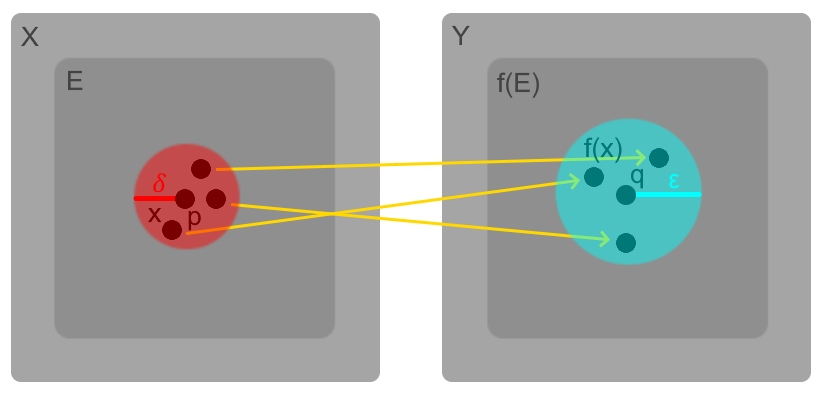
\includegraphics[scale=0.45]{Images/11.1.1.png}
    \end{figure}



    \begin{wtheorem}{Sequence definition of $\lim_{x \rightarrow p} f(x) = q$}{16cm}
        $\lim_{x \rightarrow p} f(x) = q$ if and only if
        $\lim_{n \rightarrow \infty} f(p_n) = q$ for every
        sequence \{$p_n$\} $\in$ E where $p_n \not = p$ and
        $\lim_{n \rightarrow \infty} p_n = p$
    \end{wtheorem}

    \begin{proof}
        Suppose $\lim_{x \rightarrow p} f(x) = q$.

        For $\epsilon$ $>$ 0, there is a $\delta$ $>$ 0 such that
        $d_Y(f(x),q) < \epsilon$ if x $\in$ E and $d_X(x,p) < \delta$.

        Choose \{$p_n$\} $\in$ E such that $p_n \not = p$
        and $\lim_{n \rightarrow \infty} p_n = p$.

        Then for $\delta > 0$, there is N such that for n $>$ N, then
        $d_X(p_n,p)< \delta$ so $d_Y(f(p_n),q) < \epsilon$.

        \vspace{0.2cm}

        Suppose $\lim_{x \rightarrow p} f(x) \not = q$.
        Then there is a $\epsilon$ $>$ 0 such that for every $\delta$ $>$ 0,
        there is a x $\in$ E where $d_Y(f(x),q) \geq \epsilon$, but
        $d_X(x,p) < \delta$.
        Let $\delta_n = \frac{1}{n}$ and thus, there is a \{$p_n$\}
        where $p_n \not = p$ and $\lim_{n \rightarrow \infty} p_n = p$,
        but $\lim_{n \rightarrow \infty} f(p_n) \not = q$.
    \end{proof}

    \vspace{0.5cm}



    \begin{corollary}{A limit of a function is Unique}{16cm}
        If f has a limit at p, then the limit is unique
    \end{corollary}

    \begin{proof}
        If $\lim_{x \rightarrow p} f(x) = q$, then by {\color{red} theorem 11.1.2},
        $\lim_{n \rightarrow \infty} f(p_n) = q$ for every
        \{$p_n$\} $\in$ E where $p_n \not = p$ and
        $\lim_{n \rightarrow \infty} p_n = p$.

        Thus, if there exists $\lim_{x \rightarrow p} f(x) = q'$, then there is
        a \{$p_n$\} $\in$ E where $p_n \not = p$ and
        $\lim_{n \rightarrow \infty} p_n = p$, but
        $\lim_{n \rightarrow \infty} f(p_n) = q'$ which is a contradiction.
    \end{proof}

    \vspace{0.5cm}



    \begin{wtheorem}{Properties of the Limits of Functions}{16cm}
        Let E $\subset$ X, p $\in$ E', and f(x),g(x) $\in$ $\mathbb{C}$ so 
        $\lim_{x \rightarrow p} f(x) = A$, $\lim_{x \rightarrow p} g(x) = B$
    \end{wtheorem}

    \begin{enumerate}[label=(\alph*), leftmargin=2cm, itemsep=0.1cm]
        \item $\lim_{x \rightarrow p} (f+g)(x) = A+B$
        \item $\lim_{x \rightarrow p} (fg)(x) = AB$
        \item $\lim_{x \rightarrow p} (\frac{f}{g})(x) = \frac{A}{B}$
    \end{enumerate}

    \newpage





\subsection{ Continuous Functions }

    \begin{definition}{Continuous Functions}{16cm}
        Suppose X,Y are metric spaces, E $\subset$ X, p $\in$ E, and
        f maps E into Y.

        f is {\color{lblue} continuous} at p if:
        
        \begin{adjustbox}{minipage=15cm, right, vspace=0.1cm 0cm}
            For every $\epsilon > 0$, there is a
            $\delta > 0$ such that
            for all x $\in$ E where $d_X(x,p) < \delta$, then:

            \hspace{0.5cm}
            $d_Y(f(x),f(p)) < \epsilon$
        \end{adjustbox}

        f(p) have to be defined to be continuous.

        If f is continuous at every p $\in$ E, then f is continuous on E.

        f is continuous at isolated points since regardless of $\epsilon$,
        there is a $\delta > 0$ where $d_X(x,p) < \delta$ is only x = p so
        $d_Y(f(x),f(p)) = 0 < \epsilon$.
    \end{definition}



    \begin{figure}[h]
        \centering
        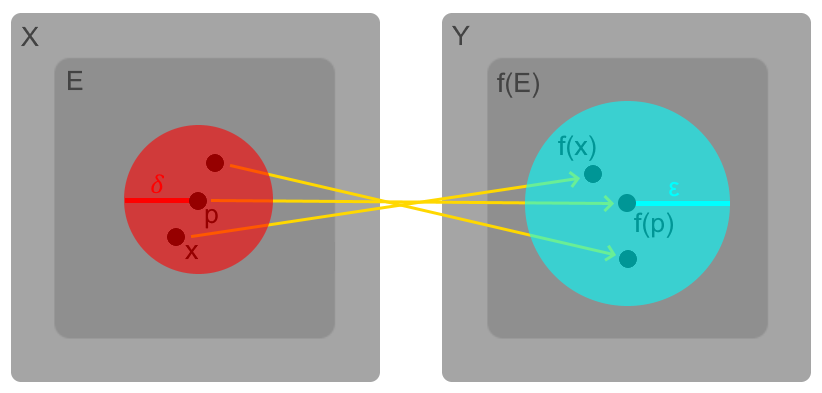
\includegraphics[scale=0.38]{Images/11.2.1.png}
    \end{figure}



    \begin{wtheorem}{Continuity at p $\rightleftharpoons$ lim f(p) = f(p)}{16cm}
        Suppose E $\subset$ X, p $\in$ E, and
        f maps E into Y. Let p $\in$ E'.

        Then f is continuous at p if and only if
        $\lim_{x \rightarrow p} f(x) = f(p)$.
    \end{wtheorem}

    \begin{proof}
        If f is continuous at p, then for every $\epsilon > 0$, there
        is a $\delta > 0$ such that $d_Y(f(x),f(p)) < \epsilon$
        for all x $\in$ E where $d_X(x,p) < \delta$.
        Thus, $\lim_{x \rightarrow p} f(x) = f(p)$.

        \vspace{0.2cm}

        If $\lim_{x \rightarrow p} f(x) = f(p)$, then for every
        $\epsilon > 0$, there is a $\delta > 0$ where $d_Y(f(x),f(p)) < \epsilon$
        for all x $\in$ E where $d_X(x,p) < \delta$.
        Thus, f is continuous at p.
    \end{proof}

    \vspace{0.5cm}



    \begin{wtheorem}{Continuity Chain Rule}{16cm}
        Suppose E $\subset$ X, f: E $\rightarrow$ Y, g: f(E) $\rightarrow$ Z,
        and h: E $\rightarrow$ Z where h(x) = g(f(x)).

        If f is continuous at p and g is continuous at f(p),
        then h is continuous at p.
    \end{wtheorem}

    \begin{proof}
        Since g is continuous at f(p), then for $\epsilon > 0$, there is a
        $\delta_1$ such that:

        \hspace{1cm}
        $d_Z(g(y),g(f(p))) < \epsilon$ for $d_Y(y,f(p)) < \delta_1$
        where y $\in$ f(E)

        Since f is continuous at p, there is a $\delta_2 > 0$ such that:

        \hspace{1cm}
        $d_Y(f(x),f(p)) < \delta_1$ for $d_X(x,p) < \delta_2$ 
        where x $\in$ E

        Thus, $d_Z(h(x),h(p))$ = $d_Z(g(f(x)),g(f(p)))$ $<$ $\epsilon$
        for $d_X(x,p)$ $<$ $\delta_2$ where x $\in$ E.

        Thus, h is continuous at p.
    \end{proof}



    \begin{figure}[h]
        \centering
        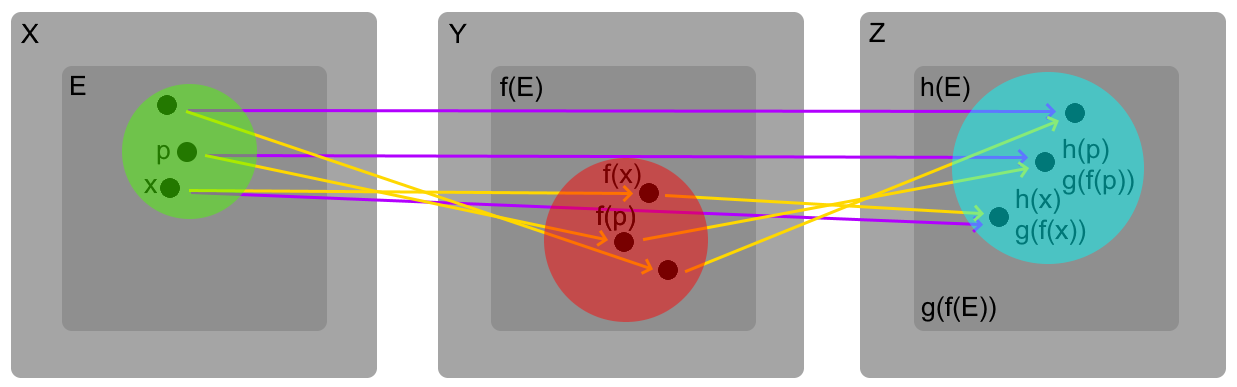
\includegraphics[scale=0.37]{Images/11.2.3.png}
    \end{figure}

    \newpage



    \begin{wtheorem}{Continuous functions map Open sets to Open sets}{16cm}
        f: X $\rightarrow$ Y is continuous on X if and only if:

        \hspace{0.5cm}
        $f^{-1}(V)$ is open in X for every open set V in Y
    \end{wtheorem}

    \begin{proof}
        Suppose f is continuous on X and V is an open set in Y.

        Suppose p $\in$ X and f(p) $\in$ V.
        Since V is open, there exists $\epsilon > 0$ such that
        y $\in$ V if $d_Y(y,f(p)) < \epsilon$.
        Since f is continuous at p, there exists $\delta > 0$ such that
        $d_Y(f(x),f(p)) < \epsilon$ for $d_X(x,p) < \delta$.
        Thus, x $\in$ $f^{-1}(V)$ for $d_X(x,p) < \delta$.

        \vspace{0.2cm}

        Suppose $f^{-1}(V)$ is open in X for every open V in Y.

        Fix p $\in$ X and $\epsilon > 0$.
        Let V be the set of all y $\in$ Y such that $d_Y(y,f(p)) < \epsilon$
        so V is open and thus, $f^{-1}(V)$ is open.
        Thus, there exists $\delta > 0$ such that x $\in$ $f^{-1}(V)$
        for $d_X(x,p) < \delta$.
        Since x $\in$ $f^{-1}(V)$, then f(x) $\in$ V
        so $d_Y(f(x),f(p)) < \epsilon$.
    \end{proof}

    \vspace{0.5cm}



    \begin{corollary}{Continuous functions map Closed sets to Closed sets}{16cm}
        f: X $\rightarrow$ Y is continuous on X if and only if:

        \hspace{0.5cm}
        $f^{-1}(C)$ is closed in X for every closed set C in Y   
    \end{corollary}

    \begin{proof}
        By {\color{red} theorem 11.2.4}, f is continuous
        if and only if $f^{-1}(V)$ is open in X for every open set V in Y.
        Let C = $V^c$.
        Since V is open, then C is closed.

        Since $f^{-1}(C)$
        = $f^{-1}(V^c)$
        = $(f^{-1}(V))^c$,
        then $f^{-1}(C)$ is closed since $f^{-1}(V)$ is open.
    \end{proof}

    \vspace{0.5cm}



    \begin{wtheorem}{Properties of Continuous functions}{16cm}
        Let f,g be complex continuous functions on X.

        Then f+g, fg, and $\frac{f}{g}$ where g $\not =$ 0 for all x $\in$ X
        are continuous on X.
    \end{wtheorem}

    \begin{proof}
        If x is an isolated point, f+g, fg, and $\frac{f}{g}$
        are continuous by definition.
        If x is a limit point, then by {\color{red} theorems 11.1.4 and 11.2.2},
        f+g, fg, and $\frac{f}{g}$ are continuous since

        \begin{itemize}[leftmargin=1cm, itemsep=0.1cm]
            \item $\lim_{x \rightarrow p} (f+g)(x)
                = \lim_{x \rightarrow p} f(x) + \lim_{x \rightarrow p} g(x)
                = f(p) + g(p)$
            \item $\lim_{x \rightarrow p} (fg)(x)
                = \lim_{x \rightarrow p} f(x) \lim_{x \rightarrow p} g(x)
                = f(p) g(p)$
            \item $\lim_{x \rightarrow p} (\frac{f}{g})(x)
                = \frac{\lim_{x \rightarrow p} f(x)}{\lim_{x \rightarrow p} g(x)}
                = \frac{f(p)}{g(p)}$
        \end{itemize}
    \end{proof}

    \vspace{0.5cm}



    \begin{ltheorem}{Continuous functions on $\mathbb{R}^k$}{1.5cm}
        \item Let $f_1,...,f_k$: X $\rightarrow$ $\mathbb{R}$ and
            f: X $\rightarrow$ $\mathbb{R}^k$ where
            f(x) = ($f_1(x)$, ... , $f_k(x)$).

            Then f is continuous if and only if $f_1,...,f_k$ are continuous.

        \item If f and g are continuous mappings of X into $\mathbb{R}^k$,
            then f + g and f $\cdot$ g are continuous on X.
    \end{ltheorem}

    \begin{proof}
        Since $|f_i(x) - f_i(y)|$
        $\leq$ $\sqrt{\sum_1^k |f_i(x) - f_i(y)|^2}$
        = $|f(x) - f(y)|$, then if f is continuous, then
        each $f_i$ is continuous and vice versa.

        \vspace{0.2cm}

        Since f,g are continuous, then by part a, each $f_i$,$g_i$ are continuous.
        Then by {\color{red} theorem 11.2.6},
        each $f_i + g_i$ and $f_i g_i$ are continuous so
        by part a, f + g and f $\cdot$ g are continuous.

        \vspace{0.2cm}

        Thus, every polynomial, rational, and absolute value function is continuous
        since polynomials are $x_1 \cdot ... \cdot x_k$ where each $x_i$
        is continuous, rationals are polynomials divided by polynomials,
        and $||x| - |y|| \leq |x - y|$ implies $|x|$ is continuous.
    \end{proof}

    \newpage





\subsection{ Continuity and Compactness }

    \begin{definition}{Bounded Functions}{16cm}
        f: E $\rightarrow$ $\mathbb{R}^k$ is {\color{lblue} bounded} if there is a
        M $\in$ $\mathbb{R}$ such that f(x) $\leq$ M for all x $\in$ E     
    \end{definition}

    \vspace{0.5cm}



    \begin{wtheorem}{Continuous functions map Compact spaces to Compact spaces}{16cm}
        Suppose f is a continuous mapping of a compact metric space X
        into a metric space Y. Then f(X) is compact.        
    \end{wtheorem}

    \begin{proof}
        Let \{$V_{\alpha}$\} be an open cover of f(X).
        Since f is continuous, then by {\color{red} theorem 11.2.4},
        each $f^{-1}(V_{\alpha})$ is open.
        Since X is compact, there is n where
        X $\subset$ $f^{-1}(V_{\alpha_1})$ $\cup$ ... $\cup$ $f^{-1}(V_{\alpha_n})$.

        Thus, f(X) $\subset$ $V_{\alpha_1}$ $\cup$ ... $\cup$ $V_{\alpha_n}$
        so f(X) is compact.
    \end{proof}



    \begin{figure}[h]
        \centering
        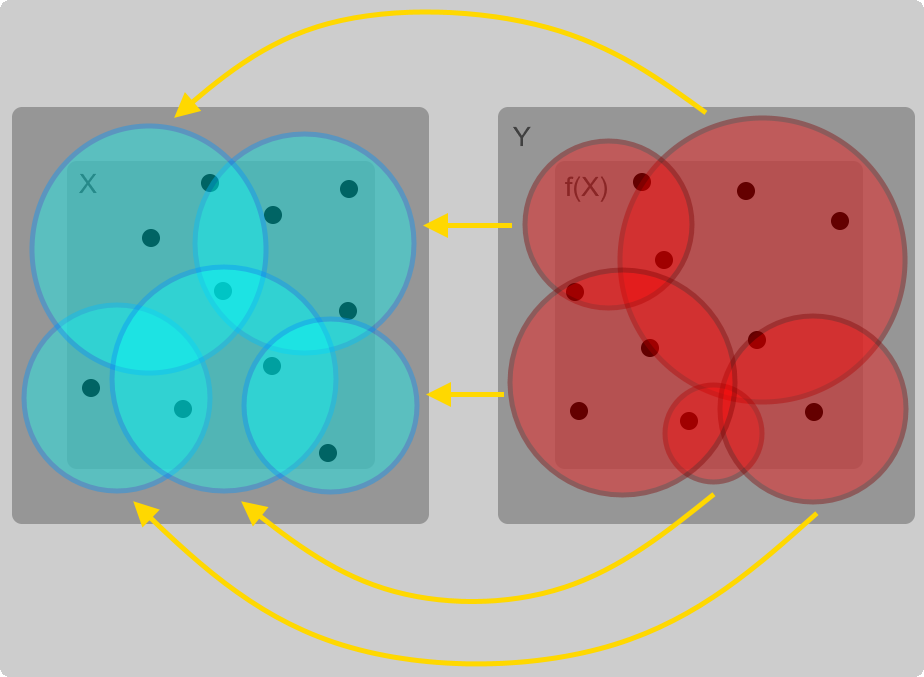
\includegraphics[scale=0.28]{Images/11.3.2.png}
    \end{figure}



    \begin{wtheorem}{Continuous functions from Compact to
    $\mathbb{R}^k$ are Bounded}{16cm}
        For continuous f: compact X $\rightarrow$ $\mathbb{R}^k$,
        then f(X) is closed and bounded
    \end{wtheorem}

    \begin{proof}
        By {\color{red} theorem 11.2.2}, f(X) is compact.
        By {\color{red} theorem 6.3.13}, f(X) is closed and bounded.
    \end{proof}

    \vspace{0.5cm}



    \begin{wtheorem}{Generalized Extreme Value Theorem}{16cm}
        Suppose f is a continuous real function of a compact metric space X
        such that M = sup$_{x \in X}$ f(x) and m = inf$_{x \in X}$ f(x).

        Then there exists p,q $\in$ X such that f(p) = M and f(q) = m.        
    \end{wtheorem}

    \begin{proof}
        By {\color{red} theorem 11.3.3}, f(X) is closed and bounded.
        Let M = $\underset{x \in X}{\text{sup}}$ f(x),
        m = $\underset{x \in X}{\text{inf}}$ f(x).

        Since f(X) is bounded, then M,m $\in$ (f(X))' and
        since f(X) is closed, then M,m $\in$ f(X).
        Thus, there exists p,q $\in$ X such that f(p) = M and f(q) = m.
    \end{proof}

    \vspace{0.5cm}



    \begin{wtheorem}{If f is continuous 1-1, then $f^{-1}$ is continuous}{16cm}
        Suppose f is a continuous 1-1 mapping of a compact metric space X
        onto a metric space Y.
        Then $f^{-1}$ is a continuous mapping of Y onto X.
    \end{wtheorem}

    \begin{proof}
        Let V be an open set in X.

        Since $V^c$ is closed and $V^c$ $\subset$ compact set X,
        then by {\color{red} theorem 6.3.5}, $V^c$ is compact.

        Thus by {\color{red} theorem 11.3.2}, f($V^c$) is a compact
        subset of Y so f($V^c$) is closed.

        Since f is 1-1 and onto, f($V^c$) = $(f(V))^c$ so f(V) is open.
        Since from any open set V in X, f(V) is open in Y, then by
        {\color{red} theorem 11.2.4}, $f^{-1}$ is continuous.
    \end{proof}

    \newpage



    \begin{definition}{Uniformly Continuous}{16cm}
        Let f: X $\rightarrow$ Y. Then f is {\color{lblue} uniformly continuous}
        on X if:
        
        \begin{adjustbox}{minipage=15cm, right, vspace=0.1cm 0cm}
            For every $\epsilon > 0$, there is a $\delta > 0$
            such that for all p,q $\in$ X where $d_X(p,q) < \delta$, then:

            \hspace{0.5cm}
            $d_Y(f(p),f(q)) < \epsilon$
        \end{adjustbox}
    \end{definition}

    \vspace{0.5cm}



    \begin{wtheorem}{Continuous functions on Compact are Uniformly continuous}{16cm}
        Let f be a continuous mapping of a compact metric space X into
        metric space Y.
        Then f is uniformly continuous on X.
    \end{wtheorem}

    \begin{proof}
        For $\epsilon > 0$, since f is continuous, then for each
        p $\in$ X, there is a $\phi(p)$ such that for all q $\in$ X
        where $d_X(q,p) < \phi(p)$, $d_Y(f(q),f(p)) < \frac{\epsilon}{2}$.

        Let J(p) be the set of all q $\in$ X where
        $d_X(q,p) < \frac{1}{2}\phi(p)$.

        Since the set of all J(p) is an open cover of X and since X is compact,
        then there is a n such that X $\subset$ J($p_1$) $\cup$ ... $\cup$ J($p_n$).
        Let $\delta$ = $\frac{1}{2}$ min( $\phi(p_1), ... , \phi(p_n)$ ) $>$ 0.

        Then for p,q $\in$ X where $d_X(p,q) < \delta$, there is a m where
        $1 \leq m \leq n$ such that p $\in$ J($p_m$) so
        $d_X(p,p_m) < \frac{1}{2} \phi(p_m)$. Thus:

        \hspace{1cm}
        $d_X(q,p_m) \leq d_X(q,p) + d_X(p,p_m) < \delta + \frac{1}{2} \phi(p_m)
        \leq \phi(p_m)$

        \hspace{1cm}
        $d_Y(f(p),f(q)) \leq d_Y(f(p),f(p_m)) + d_Y(f(p_m),f(q))
        < \frac{\epsilon}{2} + \frac{\epsilon}{2} = \epsilon$
    \end{proof}

    \vspace{0.5cm}



    \begin{wtheorem}{Continuous functions from noncompact
    $\not \rightarrow$ Uniformly continuous}{16cm}
        Let E be a noncompact set in $\mathbb{R}^1$.

        \begin{enumerate}[label=(\alph*), leftmargin=1cm, itemsep=0.1cm]
            \item There exists a continuous function which is not bounded
            
            \item There exists a continuous, bounded function which is
            has no maximum
            
            \item If E is bounded, there exists a continuous function which
            is not uniformly continuous
        \end{enumerate}
    \end{wtheorem}
    
    \begin{proof}
        Suppose E is bounded so there is a $x_0$ $\in$ E', but $x_0$ $\not \in$ E.

        Consider f(x) = $\frac{1}{x - x_0}$ which is continuous on E, but unbounded.

        For $\epsilon > 0$ and $\delta > 0$, there is a x $\in$ E such that
        $|x - x_0| < \delta$.
        Take t close enough to $x_0$ so $|f(t) - f(x_0)| > \epsilon$,
        but $|t - x| < \delta$.
        Thus, f is not uniformly continuous.

        \vspace{0.2cm}

        Consider g(x) = $\frac{1}{1 + (x - x_0)^2}$ which is continuous on E
        and bounded since g(x) $\in$ (0,1).

        Since sup$_{x \in E}$ g(x) = 1, but g(x) $<$ 1 for all x $\in$ E, then
        g has no maximum on E.
    \end{proof}

    \vspace{0.5cm}





\subsection{ Continuity and Connectedness }

    \begin{wtheorem}{Continuous functions map Connected spaces
    to Connected spaces}{16cm}
        If f is a continuous mapping of X into Y and E is a connected
        subset of X, then f(E) is connected.
    \end{wtheorem}

    \begin{proof}
        Suppose f(E) = A $\cup$ B where A and B are nonempty separated
        subsets of Y.
        
        Let G = E $\cap$ $f^{-1}(A)$ and H = E $\cap$ $f^{-1}(B)$.
        Then E = G $\cup$ H.

        Since A $\subset$ $\overline{A}$, G $\subset$ $f^{-1}(\overline{A})$.
        Since f is continuous, then $f^{-1}(\overline{A})$ is closed so
        $\overline{G}$ $\subset$ $f^{-1}(\overline{A})$.
        Thus, f($\overline{G}$) $\subset$ $\overline{A}$.

        Since f(H) = B and $\overline{A}$ $\cap$ B is empty,
        $\overline{G}$ $\cap$ H is empty.
        Similarily, G $\cap$ $\overline{H}$ is empty so G and H are separated
        which contradicts that E = G $\cup$ H is connected.
    \end{proof}

    \newpage



    \begin{wtheorem}{Generalized Intermediate Value Theorem}{16cm}
        Let f be a continuous real function on [a,b]. If f(a) $<$ c $<$ f(b),
        then there exists x $\in$ (a,b) such that f(x) = c.
    \end{wtheorem}

    \begin{proof}
        Since [a,b] is connected, then by {\color{red} theorem 11.4.1},
        f([a,b]) is a connected subset of $\mathbb{R}^1$.

        Thus, by {\color{red} theorem 7.2.2}, any c where f(a) $<$ c $<$ f(b)
        is c $\in$ f(x) for some x $\in$ [a,b].
    \end{proof}

    \vspace{0.5cm}





\subsection{ Discontinuities }

    \begin{definition}{Right and Left Limits}{16cm}
        \small
        Let f be defined on (a,b).
        
        \vspace{0.2cm}

        Then for any x where x $\in$ [a,b), f(x+) = q if:
        
        \hspace{1cm}
        f($t_n$) $\rightarrow$ q as n $\rightarrow$ $\infty$
        for all sequences \{$t_n$\} in (x,b) such that $t_n$ $\rightarrow$ x.

        \vspace{0.2cm}

        Then for any x where x $\in$ (a,b], f(x-) = q if:
        
        \hspace{1cm}
        f($t_n$) $\rightarrow$ q as n $\rightarrow$ $\infty$
        for all sequences \{$t_n$\} in (a,x) such that $t_n$ $\rightarrow$ x.

        \vspace{0.2cm}

        Then $\lim_{t \rightarrow x}$ f(t) exists if and only if
        f(x-) = f(x+) = $\lim_{t \rightarrow x}$ f(t).
    \end{definition}

    \vspace{0.5cm}



    \begin{definition}{Types of Discontinuities}{16cm}
        \small
        If f is discontinuous at x, but f(x+) and f(x-) exists,
        then f have a simple discontinuity of the first kind else
        it is a discontinuity of the second kind.

        Thus, a {\color{lblue} simple discontinuity} is either:

        \begin{itemize}[leftmargin=1cm, itemsep=0.1cm]
            \item f(x-) $\not = $ f(x+)
            
            \item f(x-) = f(x+) $\not =$ f(x) 
        \end{itemize}
    \end{definition}

    \vspace{0.5cm}





\subsection{ Monotonic Functions }

    \begin{definition}{Monotonic}{16cm}
        \small
        f: (a,b) $\rightarrow$ $\mathbb{R}$ is monotonically increasing
        if f(x) $\leq$ f(y) for $a < x < y < b$.

        f: (a,b) $\rightarrow$ $\mathbb{R}$ is monotonically decreasing
        if f(x) $\geq$ f(y) for $a < x < y < b$.        
    \end{definition}

    \vspace{0.5cm}



    \begin{wtheorem}{Right and Left Limits of Monotonics on (a,b)}{16cm}
        Let f be monotonically increasing on (a,b).

        Then f(x+) and f(x-) exists at every x $\in$ (a,b) where:

        \hspace{1cm}
        sup$_{t \in (a,x)}$ f(t)
        = f(x-)
        $\leq$ f(x)
        $\leq$ f(x+)
        = inf$_{t \in (x,b)}$ f(t)

        Furthermore, for $a < x < y < b$, f(x+) $\leq$ f(y-).

        Properties analogous for monotonically decreasing functions.
    \end{wtheorem}

    \begin{proof}
        \small
        Since f is monotonically increasing, then for t $\in$ (a,x),
        f(t) is bounded above by f(x) and thus, by the least upper bounded
        property, sup$_{t \in (a,x)}$ f(t) exists.

        For $\epsilon > 0$, there exists a $\delta > 0$ such that
        sup$_{t \in (a,x)}$ f(t) - $\epsilon$
        $<$ f(x - $\delta$)
        $\leq$ sup$_{t \in (a,x)}$ f(t)
        for a $<$ x - $\delta$ $<$ x.
        Since f(x - $\delta$) $\leq$ f(t) $\leq$ sup$_{t \in (a,x)}$ f(t)
        for t $\in$ (x-$\delta$,x), then
        $|f(t) - \text{sup}_{t \in (a,x)} f(t)| < \epsilon$ for
        t $\in$ (x-$\delta$,x) so f(x-) = sup$_{t \in (a,x)}$ f(t).

        For $\epsilon > 0$, there exists a $\delta > 0$ such that
        inf$_{t \in (x,b)}$ f(t)
        $<$ f(x + $\delta$)
        $\leq$ inf$_{t \in (x,b)}$ f(t) + $\epsilon$
        for x $<$ x + $\delta$ $<$ b.
        Since f(x + $\delta$) $\geq$ f(t) $\geq$ inf$_{t \in (x,b)}$ f(t)
        for t $\in$ (x,x+$\delta$), then
        $|f(t) - \text{inf}_{t \in (x,b)} f(t)| < \epsilon$ for
        t $\in$ (x,x+$\delta$) so f(x+) = inf$_{t \in (x,b)}$ f(t).

        Thus,
        sup$_{t \in (a,x)}$ f(t) = f(x-)
        $\leq$ f(x)
        $\leq$ f(x+) = inf$_{t \in (x,b)}$ f(t).

        If $a < x < y < b$, then:

        \hspace{1cm}
        f(x+) = inf$_{t \in (x,b)}$ f(t)
        = inf$_{t \in (x,y)}$ f(t)
        $\leq$ sup$_{t \in (x,y)}$ f(t)
        = sup$_{t \in (a,y)}$ f(t)
        = f(y-)
    \end{proof}

    \newpage



    \begin{corollary}{Monotonics can only have Simple discontinuities}{16cm}
        Monotonic functions have no discontinuities of the second kind
    \end{corollary}

    \begin{proof}
        By {\color{red} theorem 11.6.2}, f(x-) and f(x+) exists and thus,
        f can only have simple discontinuities and not discontinuities
        of the second kind.
    \end{proof}

    \vspace{0.5cm}



    \begin{wtheorem}{Discontinuities of Monotonics is at most Countable}{16cm}
        Let f be monotonic on (a,b).
        Then the set of points of (a,b) where f is discontinuous is
        at most countable.
    \end{wtheorem}

    \begin{proof}
        Suppose f is increasing.
        Let E be the set of points where f is discontinuous.
        Then for x $\in$ E, there is a rational r(x) where
        f(x-) $<$ r(x) $<$ f(x+).
        
        Then for $x_1$ $<$ $x_2$, by {\color{red} theorem 11.6.2},
        f($x_1$+) $\leq$ f($x_2$-). Then:

        \hspace{1cm}
        f($x_1$-) $<$ r($x_1$) $<$ f($x_1$+)
        $\leq$ f($x_2$-) $<$ r($x_2$) $<$ f($x_2$+)

        Thus, r($x_1$) $\not =$ r($x_2$) if $x_1$ $\not =$ $x_2$.

        Since there is a 1-1 correspondence between E and a subset
        of rational numbers which is countable, then E is at most countable.

        If f is decreasing, proof is analogous.
    \end{proof}

    \vspace{0.5cm}





\subsection{ Infinite Limits / Limits at Infinity }

    \begin{definition}{Neighborhoods in the Extended Reals}{16cm}
        For any real c, a neighborhood of $+\infty$ = (c,$+\infty$).

        For any real c, a neighborhood of $-\infty$ = ($-\infty$,c).        
    \end{definition}

    \vspace{0.5cm}



    \begin{definition}{Infinite Limits}{16cm}
        Let real function f be defined on E $\subset$ $\mathbb{R}$.

        Then f(t) $\rightarrow$ A as t $\rightarrow$ x where A and x
        are extended reals if:
        
        \begin{adjustbox}{minipage=15cm, right, vspace=0.1cm 0cm}
            For every neighborhood U of A,
            there is a neighborhood V of x such that V $\cap$ E $\not =$ $\emptyset$
            and f(t) $\in$ U for all t $\in$ V $\cap$ E where t $\not =$ x.
        \end{adjustbox}        
    \end{definition}

    \vspace{0.5cm}



    \begin{wtheorem}{Properties on functions of Infinite limits}{16cm}
        Let f,g be defined on E $\subset$ $\mathbb{R}$ where
        f(t) $\rightarrow$ A and g(t) $\rightarrow$ B as t $\rightarrow$ x.
    \end{wtheorem}

    \begin{enumerate}[label=(\alph*), leftmargin=2cm, itemsep=0.1cm]
        \item If f(t) $\rightarrow$ A', then A' = A.
        
        \item (f+g)(t) $\rightarrow$ A + B
        
        \item (fg)(t) $\rightarrow$ AB
        
        \item $\frac{f}{g}$(t) $\rightarrow$ $\frac{A}{B}$
    \end{enumerate}




    